%! Author = aybehrouz



Every transaction in the Argennon blockchain starts with an \texttt{invoke\_external} instruction which calls a
special method from the root smart contract. This method will transfer the proposed fee of the transaction in ARGs
from a sender account to the fee sink accounts. Argennon has two fee sink accounts: \texttt{execFeeSink} collects
execution fees and \texttt{dbFeeSink} collects fees for ZK-EDB servers. The Protocol decides how to distribute the
transaction fee between these two fee sink accounts.

When a block is added to the blockchain, the proposer of that block will receive a share of the block fees.
Consequently, a block proposer is always incentivized to include more transactions in his block. However, if he
puts too many transactions in his block and the validation of the block becomes too difficult, some validators
may not be able to validate all transactions on time. If a validator can not validate a block in the required
time, he will consider the block invalid. So, when a proposed block contains too many transactions, the network
may reach consensus on another block, and the proposer of that block will not receive any fees. As a result, a
proposer is incentivized to use network transaction capacity optimally.

On the other hand, we believe that the proposer does not have enough incentives for optimizing the storage size
of the transaction set. Therefore, we require that \textbf{the size of the transaction set of every block in
bytes be lower than a certain threshold.}

Validators need to spend resources for validating transactions. When a validator starts the emulation of the AVM
to validate a transaction, solely from the code he can't predict the time the execution will finish. This will
give an adversary an opportunity to attack the network by broadcasting transactions that never ends. Since,
validators can not finish the execution of these transactions, the network will not be able to charge the
attacker any fees, and he would be able to waste validators resources for free.

To mitigate this problem, we require that every transaction specify a cap for all the resources it needs. This
will include memory, network and processor related resources. Also, the protocol defines an execution cost for
every AVM instruction reflecting the amount of resources its emulation needs. This will define a standard way for
measuring the execution cost of any \texttt{avmCall} transaction. Every \texttt{avmCall} transaction is required
to specify a maximum execution cost. If during emulation it reaches this maximum cost, the transaction will be
considered failed and the network can receive the proposed fee of that transaction.


In Argennon \emph{light} nodes do not keep a full copy of the AVM storage and for emulating the Argennon Virtual Machine
( i.e.~validating transactions) they need to connect to a ZK-EDB and retrieve the required pages.
Because light node need to be able to validate block certificates, they usually cache a large part of the staking
database, and keep their cache updated to make sure they can keep themselves in sync with the blockchain.


On the other hand, nodes that are chosen to be validators, for validating a new block, need to emulate the
execution of the Argennon Virtual Machine. To do so, first they retrieve all storage pages they
need from available ZK-EDBs. Then, they emulate the execution of AVM instructions and validate all the
transactions included in the new block. This will modify some pages of the AVM storage, so they update the ZK-EDB
commitments based on the modified pages and verify the commitments included in the new block. Validators also
calculate and verify the commitment to the new block's transaction set.

\note{Validators do not need to write the modified pages back to ZK-EDB servers. ZK-EDB servers will receive the new
block, and they will update their database by emulating the AVM execution.}


The only information that all Argennon nodes are required to store is \textbf{the most recent block} of the Argennon
blockchain.
We store the commitment of this
transaction set in every block, but we don't keep the set itself. To be able to detect replay attacks, we require
every signature that a user creates to have a nonce. This nonce consists of the issuance round of the signature
and a sequence number: \texttt{(issuance,\ sequence)}. When a user creates more than one signature in a round, he
must sequence his signatures starting from 0 (i.e.~the sequence number restarts from 0 in every round). We define
a maximum lifetime for signatures, so a signature is invalid if \texttt{currentRound - issuance > maxLifeTime} or
if a signature of the same user with a bigger or equal nonce is already used
(i.e.~is recorded in the blockchain). A nonce is bigger than another nonce if it has an older issuance. If two
nonces have an equal issuance, the nonce with the bigger sequence number will be considered bigger.

To be able to detect invalid signatures, we keep the maximum nonce of used digital signatures per user. When the
difference between \texttt{issuance} component of this nonce and the current round becomes bigger than the
maximum allowed lifetime of a signature, this information can be safely deleted. \textbf{As a result, we will not
have the problem of "un-removable empty accounts" like Ethereum.}



In our system a newly created account will not have voting power for some time, no matter how high its
balance is. While this is a desirable property, in case a large proportion of total system tokens are
transferred to newly created accounts, it can result in too much voting power for older accounts. This may decrease
the degree of decentralization in our system.

However, this situation is easily detectable by comparing the total stake of the system with the total balance of
users. If after confirming a block the total stake of the system goes too low and we have:
\[
    \sum_{u}S_{u,t} < \gamma \sum_{u}B_{u,t}
\]
The protocol will perform a \emph{time shift} in the system: the time step of the system
will be incremented for \(m\) steps while no blocks will be confirmed. This will increase the value of \(M_{u,t}\)
for new accounts with a non-zero balance, giving them more influence in the agreement protocol.

For calculating the value of \(m\) which determines the amount of time shift in the system, we should note that when
\(B_{u,t} = B_{u, t-1} = B_u\), we can derive a simple recursive rule for the stake of a user:
\[
    S_{u,t} = (1 - \alpha) S_{u,t-1} + \alpha B_u
\]
Therefore, we have:
\[
    \sum_{u}S_{u,t} = (1 - \alpha) \sum_{u}S_{u,t - 1} + \alpha \sum_{u}B_u
\]
This equation shows that when the balance of users is not changing over time the total stake of the system is the
exponential average of the total ARGs of the system. Consequently, when we shift the time for \(m\) steps, we can
calculate the new total stake of the system from the following equation:

\[
    \sum_{u}S_{u,t+m} = (1 - \alpha)^{m}\sum_{u}S_{u,t} + [1 - (1 - \alpha)^{m}]\sum_{u}B_u
\]
Hence, if we want to increase the total stake of the system from \(\gamma \sum_{u}B_u\) to \(\lambda \sum_{u}B_u\),
we can obtain \(m\) from the following formula, assuming \(\alpha\) is small enough:
\[
    m = \frac{1}{\alpha} \ln \left(\frac{1 - \gamma}{1 - \lambda}\right)
\]

An Argennon block certificate is not a part of the block data. This means that the Argennon blockchain does not have a
unique certificate sequence. Any node may have its own valid certificate sequence based on the signatures
it has collected over time.




\subsection{Memory Shards}\label{subsec:memory-shards}

In order to further increase the concurrency level of Argennon, we can divide the AVM memory into \emph{shards}.
Each memory shard can be persisted using a different ZK-EDB, hence having its own commitment. Then, the
consensus on new values of the commitment of any shard can be achieved by a different voting committee.

If a transaction does not modify a memory shard and in the transaction ordering of the block it comes after
any transaction which modifies that shard, then the execution of that transaction is not needed for calculating
the new commitment of the shard. Consequently, the voting committee of that memory shard can safely ignore such a
transaction. The execution DAG of transactions can be used for finding and pruning these transactions as
we see in Algorithm~\ref{alg:prune_dag}.

%##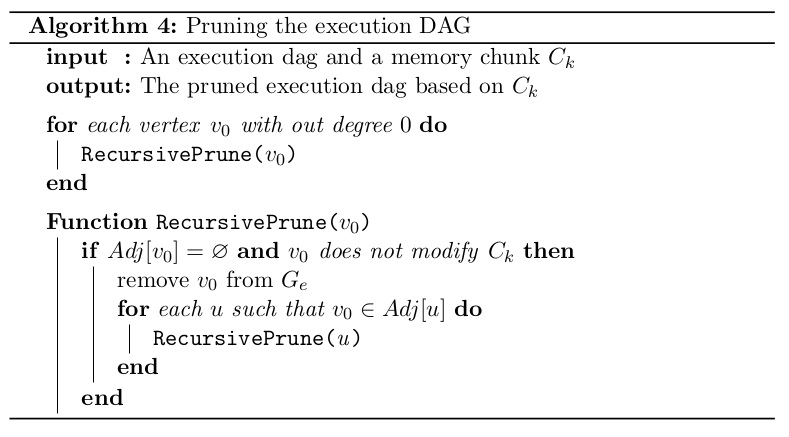
\includegraphics[width=17cm]{../img/Alg4s.png}
\begin{algorithm}
    \DontPrintSemicolon
    \SetKwData{V}{$v_0$}\SetKwData{Graph}{$G_e$}\SetKwData{Shard}{$Sh_k$}\SetKwData{Txns}{$T$}
    \SetKwFunction{RPrune}{RecursivePrune}
    \SetKwProg{Fn}{Function}{}{}
    \SetKwInOut{Input}{input}\SetKwInOut{Output}{output}
    \Input{An execution dag \Graph and a memory shard \Shard}
    \Output{The pruned execution dag based on \Shard}
    \BlankLine
    \For{each vertex \V with out degree $0$}
    {
        \RPrune{\V}\;
    }
    \BlankLine
    \Fn{\RPrune{\V}}
    {
        \If{$Adj[\V] = \varnothing$ {\bf and} \V does not modify \Shard}
        {
            remove \V from \Graph\;
            \For{each $u$ such that edge $(u,\V)$ was in \Graph}
            {
                \RPrune{u}\;
            }
        }
    }
    \caption{Pruning an execution DAG}\label{alg:prune_dag}
\end{algorithm}

If we choose shards in a way that most transactions only modify memory locations of one shard,
likely many transactions of a block only need to be validated by one voting committee and can be validated in
parallel by different committees.

Because the voting committees are selected by random sampling, by choosing large enough samples we can make sure
that having multiple voting committees will not change the security properties of the Argennon agreement protocol.


If a block receives a "reject" certificate from its committee or does not receive a certificate
after \texttt{certificateTimeOut} period of time, it will be conditionally validated by \textbf{all} validators. If
it does not receive an "accept" certificate, the validators initiate the recovery protocol.



A valid fork block
A validator issues
an "accept" certificate for a fork block at position $b + 1$ (which forks the blockchain at block $b$), if:
\begin{itemize}
    \item the fork block is signed by the reserve committee of delegates and block $b$ is its parent.
    \item the block $b$ has a valid certificate from validators.
    \item the fork block contains a valid fork request according to the staking database of block $b$.
    \item the validator has not signed a certificate for block $b + 1$.
\end{itemize}

will force the fork, in the sense that any validator after receiving it considers the forked chain as the new
valid chain.
Emergency forking may discard at max one block with a valid validator's certificate
from the blockchain, in the worst case scenario.



\subsection{Memory Allocation and De-allocation Fee}\label{subsec:memory-allocation-and-de-allocation}

Every $k$ round the protocol chooses a price per byte for AVM memory. When a smart contract executes a heap
allocation instruction, the protocol will automatically deduce the cost of the allocated memory from the ARG
address of the smart contract.

To determine the price of AVM memory, Every $k$ round, the protocol calculates \texttt{dbFee} and
\texttt{memTraffic} values. \texttt{dbFee} is the aggregate amount of collected database fees, and
\texttt{memTraffic} is the total memory traffic of the system. For calculating the memory traffic of the system
the protocol considers the total size of all the memory pages that were accessed for either reading or writing
during a time period. These two values will be calculated for the last $k$ rounds and the price per byte of
AVM memory will be a linear function of \texttt{dbFee/memTraffic}

When a smart contract executes a heap de-allocation instruction, the protocol will refund the cost of
de-allocated memory to the smart contract. Here, the current price of AVM memory does not matter and the protocol
calculates the refunded amount based on the average price the smart contract had paid for that allocated memory.
This will prevent smart contracts from profit taking by trading memory with the protocol.



If the pc register points to an \texttt{invoke} instruction, the current method completes abruptly too.
including its local frame and operand stack, with the \texttt{pc} register appropriately restored and incremented
to skip past the method invocation instruction. If the current call stack is empty the next call stack in the call
stack queue will be used for continuing the execution, and when there are no call stacks left in the queue the
current execution session ends.

When an exception is thrown
Algorithm~\ref{alg:Abrupt} is used to restore the state of the AVM heap.

\begin{algorithm}
    \DontPrintSemicolon
    \SetKwData{Heap}{Heap}\SetKwData{Stack}{CallStack}
    \SetKwFunction{Discard}{Discard}\SetKwFunction{Pop}{pop}\SetKwFunction{Restore}{Restore}
    \SetKwProg{Fn}{Function}{}{}

    \While{\Stack is not empty}
    {
        \Stack.\Pop{}\;
        \eIf{\Stack is not empty \textbf{and} $\Stack[head].pc \rightarrow catch$}
        {
            \Heap.\Restore{}\;
        }{
            \Heap.\Discard{}\;
        }
    }
    \Heap.\Restore{}\;
    \caption{Abrupt method completion}\label{alg:Abrupt}
\end{algorithm}

A closer investigation of Algorithm~\ref{alg:Abrupt} shows that when an invocation which was made by
a \texttt{spawn} instruction completes abruptly, the heap snapshot that was saved before the start of the
execution of the first call stack of the execution session is restored. Since the root
smart contract calls \texttt{Heap.Save()} function before spawning the requested method, this means
that all changes made to the AVM heap during the execution session will be restored, but the changes made by
the root smart contract including the transferring of the transaction fee will not be restored. See
Section~\ref{sec:execution-sessions} for more details.


